\begin{frame}[fragile]

  {\Huge Vendor and Independent Profiling GUIs}

  \vspace{10pt}

  {\large Connector tools translating Kokkos instrumentation.}

  \vspace{20pt}

  \textbf{Learning objectives:}
  \begin{itemize}
    \item {Understand what connectors provide}
    \item {Understand what tools are available}
  \end{itemize}

  \vspace{-20pt}

\end{frame}

%==========================================================================

\begin{frame}[fragile]{Using Third Party Tools}
Kokkos Tools can also be used to interface and augment existing profiling tools.

\begin{itemize}
  \item Provide context information like Kernel names
  \item Turn data collection on and off in a tool independent way
\end{itemize}

\vspace{10pt}
There are two ways this happens:
\begin{itemize}
  \item Load a specific connector tool like \texttt{nvtx-connector}
  \begin{itemize}
     \item For example for Nsight Compute and VTune
  \end{itemize}
  \item Tools themselves know about Kokkos instrumentation
  \begin{itemize}
     \item For example Tau
  \end{itemize}
\end{itemize}
\end{frame}

%==========================================================================

\begin{frame}[fragile]{Connecting to Tools - Nsight Compute}
\textbf{Use the \texttt{nvtx-connector} to interact with NVIDIA tools}

\vspace{10pt}
Translates KokkosP hooks into NVTX instrumentation
\begin{itemize}
\item Works with all NVIDIA tools which understand NVTX
\item Translates Regions and Kernel Dispatches
\end{itemize}

\pause
\vspace{10pt}
Initially wasn't very useful since regions are shown independently of kernels

\pause
\vspace{15pt}
\textbf{But CUDA 11 added renaming of Kernels based on Kokkos User feedback!}
\end{frame}

\begin{frame}[fragile]{Connecting to Tools - Nsight Compute}
  To enable kernel renaming you need to:
  \begin{itemize}
    \item Load the nvprof-connector via setting \texttt{KOKKOS\_TOOLS\_LIBS} in the run configuration.
    \item Go to \texttt{Tools > Preferences > Rename CUDA Kernels by NVTX} and set it on.
  \end{itemize}

  This does a few things:
  \begin{itemize}
    \item User Labels are now used as the primary name.
    \item You can still expand the row to see which actual kernels are grouped under it.
    \begin{itemize}
      \item For example if multiple kernels have the same label
    \end{itemize}
    \item The bars are now named \texttt{Label/GLOBAL\_FUNCTION\_NAME}.
  \end{itemize}
  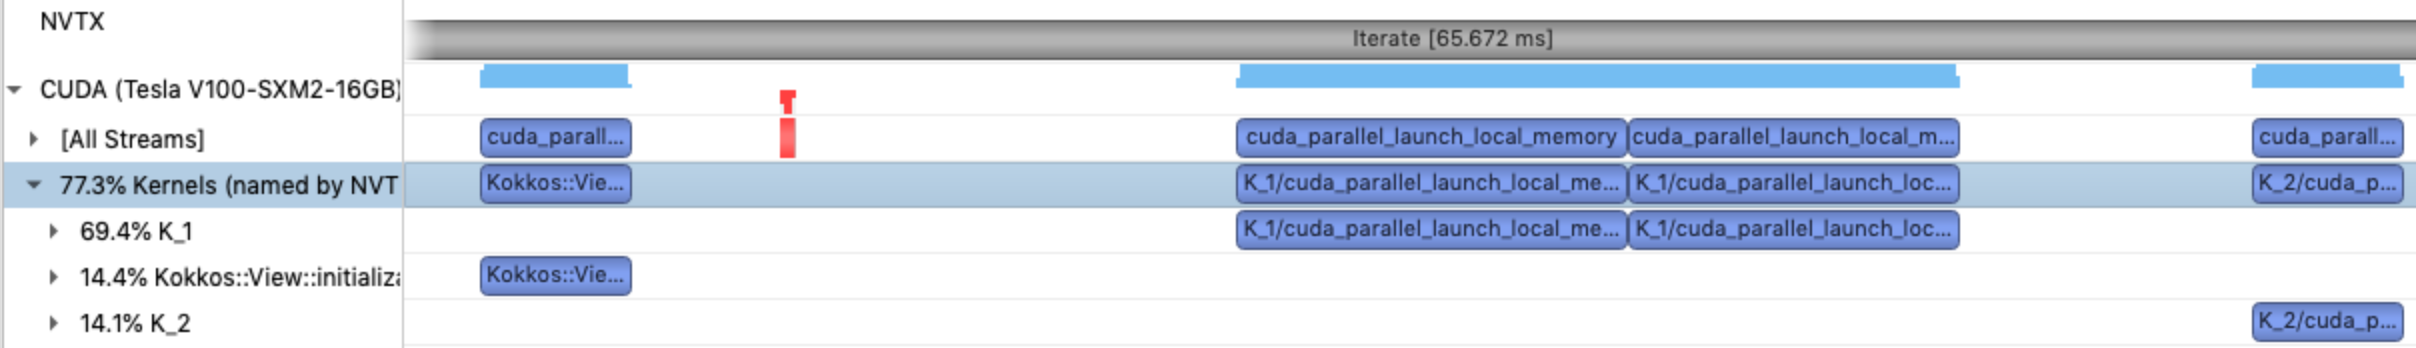
\includegraphics[width=\textwidth]{../figures/tools-simple-example-nvprof-zoomin.png}
\end{frame}



%==========================================================================

\begin{frame}[fragile]{Connecting to Tools - Vtune}
  To enable kernel renaming you need to:
  \begin{itemize}
    \item Load the vtune-connector via setting \texttt{KOKKOS\_TOOLS\_LIBS} in the run configuration.
    \item Choose the \texttt{Frame Domain / Frame / Function / Call Stack} grouping in the bottom up panel.
  \end{itemize}

  This does a few things:
  \begin{itemize}
    \item User Labels are now used as the primary name.
    \item You can expand to see individual kernel invocations
    \item You can dive further into an individual kernel invocation to see function calls within.
    \item Focus in on a kernel or individual invocation and do more detailed analysis. 
  \end{itemize}

  Also available: vtune-focused-connector:
  \begin{itemize}
    \item Used in conjunction with kernel-filter tool.
    \item Restricts profiling to a subset of kernels.
  \end{itemize}
\end{frame}

%==========================================================================

\begin{frame}[fragile]{Connecting to Tools - Vtune}
  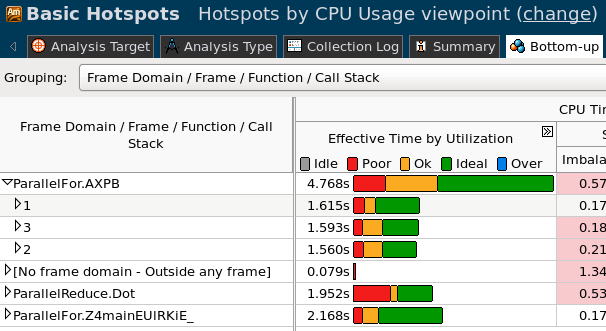
\includegraphics[width=\textwidth]{../figures/tools-vtune-example}

\end{frame}

%==========================================================================

\begin{frame}[fragile]{Connecting to Tools - Tau}
\textbf{TAU is a widely used Profiling Tool supporting most platforms.}

\vspace{5pt}
Tau supports:
\begin{itemize}
  \item profiling
  \item sampling
  \item tracing
\end{itemize}

\textbf{You do not need a connector tool for Tau!}

\vspace{5pt}
To enable TAU's Kokkos integration simply
\begin{itemize}
  \item \href{https://www.cs.uoregon.edu/research/tau/downloads.php}{Download} and install TAU
  \item Launch your program with \texttt{tau\_exec} (which will set \texttt{KOKKOS\_TOOLS\_LIBS} for you)
\end{itemize}

For questions contact tau-users@cs.uoregon.edu

\end{frame}

%==========================================================================

\begin{frame}[fragile]{Connecting to Tools - Tau}

Tau will use Kokkos instrumentation to display names and regions as defined by Kokkos:

	\vspace{10pt}
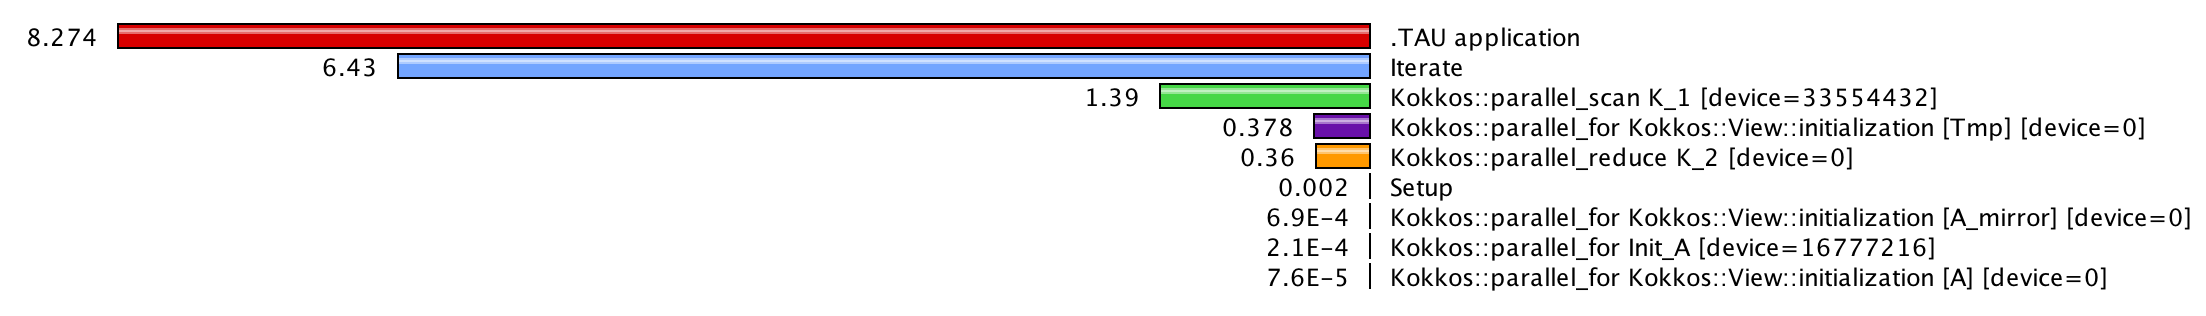
\includegraphics[width=\textwidth]{../figures/tools-simple-example-tau.png}
\end{frame}

\begin{frame}[fragile]{More Info on TAU}

\begin{center}
	In-depth tutorial: \url{http://www.nic.uoregon.edu/~khuck/kokkos/2024-Kokkos-Tuning-Tutorial/2024-Kokkos-Tools-Tutorial-TAU.pdf} 
\end{center}
	\begin{center} 
        Repo: \url{https://github.com/UO-OACISS/tau2} \\
	Contact: \url{tau-users@cs.uoregon.edu}
	\end{center} 
\end{frame}
%==========================================================================
\begin{frame}[fragile]{Timemory}
  \href{https://github.com/NERSC/timemory}{Timemory} is a modular toolkit provided by NERSC that aims to
  simplify the creation of performance analysis tools by providing a common design pattern
  of classes which encapsulate how to perform a start+stop/sample/entry of "something". 
  Each of these components (from timers to HW counters to other profilers) can be used 
  individually with zero overhead from the library. 
  It also provides wrappers and utilities for handling multiple components generically, data storage, 
  writing JSON, comparing outputs, etc. 

  \vspace{1em}
  As a by-product this design, the library
  provides an large set of individual profiling libraries whose usage comes with
  the same ease as using the simple-timer tool: setting \texttt{KOKKOS\_TOOLS\_LIBS}. 
%  \href{https://github.com/NERSC/timemory}{Timemory} is another multi architecture profiling tool.
%	
%Timemory provides:
%\begin{itemize}
%  \item a wide set of measurement capabilities.
%  \item avoid complicated environment variables.
%  \item different connector libraries for different tasks.
%  \item unique capabilities such as simultaneous CPU/GPU roofline modeling.
%\end{itemize}
%
%As with other Kokkos tools to use it:
%\begin{itemize}
%  \item	build the tools
%  \item set \texttt{KOKKOS\_TOOLS\_LIBS}
%\end{itemize}
%
\end{frame}


\begin{frame}[fragile]{Timemory}
  \begin{itemize}
  \item It also provides novel capabilities other tools don't, like simultaneous CPU/GPU
    roofline modeling. 
  \item The usage here is simple:
  \begin{itemize}
  \item \lstinline|spack install timemory +kokkos_tools +kokkos_build_config| \\
     \lstinline|[+mpi +cuda +cupti +papi +caliper ...]|
  \item Wait 3 months while spack builds every software package ever from scratch
  \item In \lstinline|<PREFIX>/lib/timemory/kokkos_tools/| there will be 5 to 30+ 
  Kokkos profiling libraries
  \end{itemize}
  \item Roofline modeling requires one additional setup
  \begin{itemize}
  \item \lstinline|timemory-roofline -T "TITLE" -t gpu_roofline -- <CMD>|
  \item Where everything after \lstinline|--| is just running your application
  \end{itemize}
  \item For more information: \url{https://github.com/NERSC/timemory}
  \end{itemize}
\end{frame}

\begin{frame}[fragile]{Timemory}
  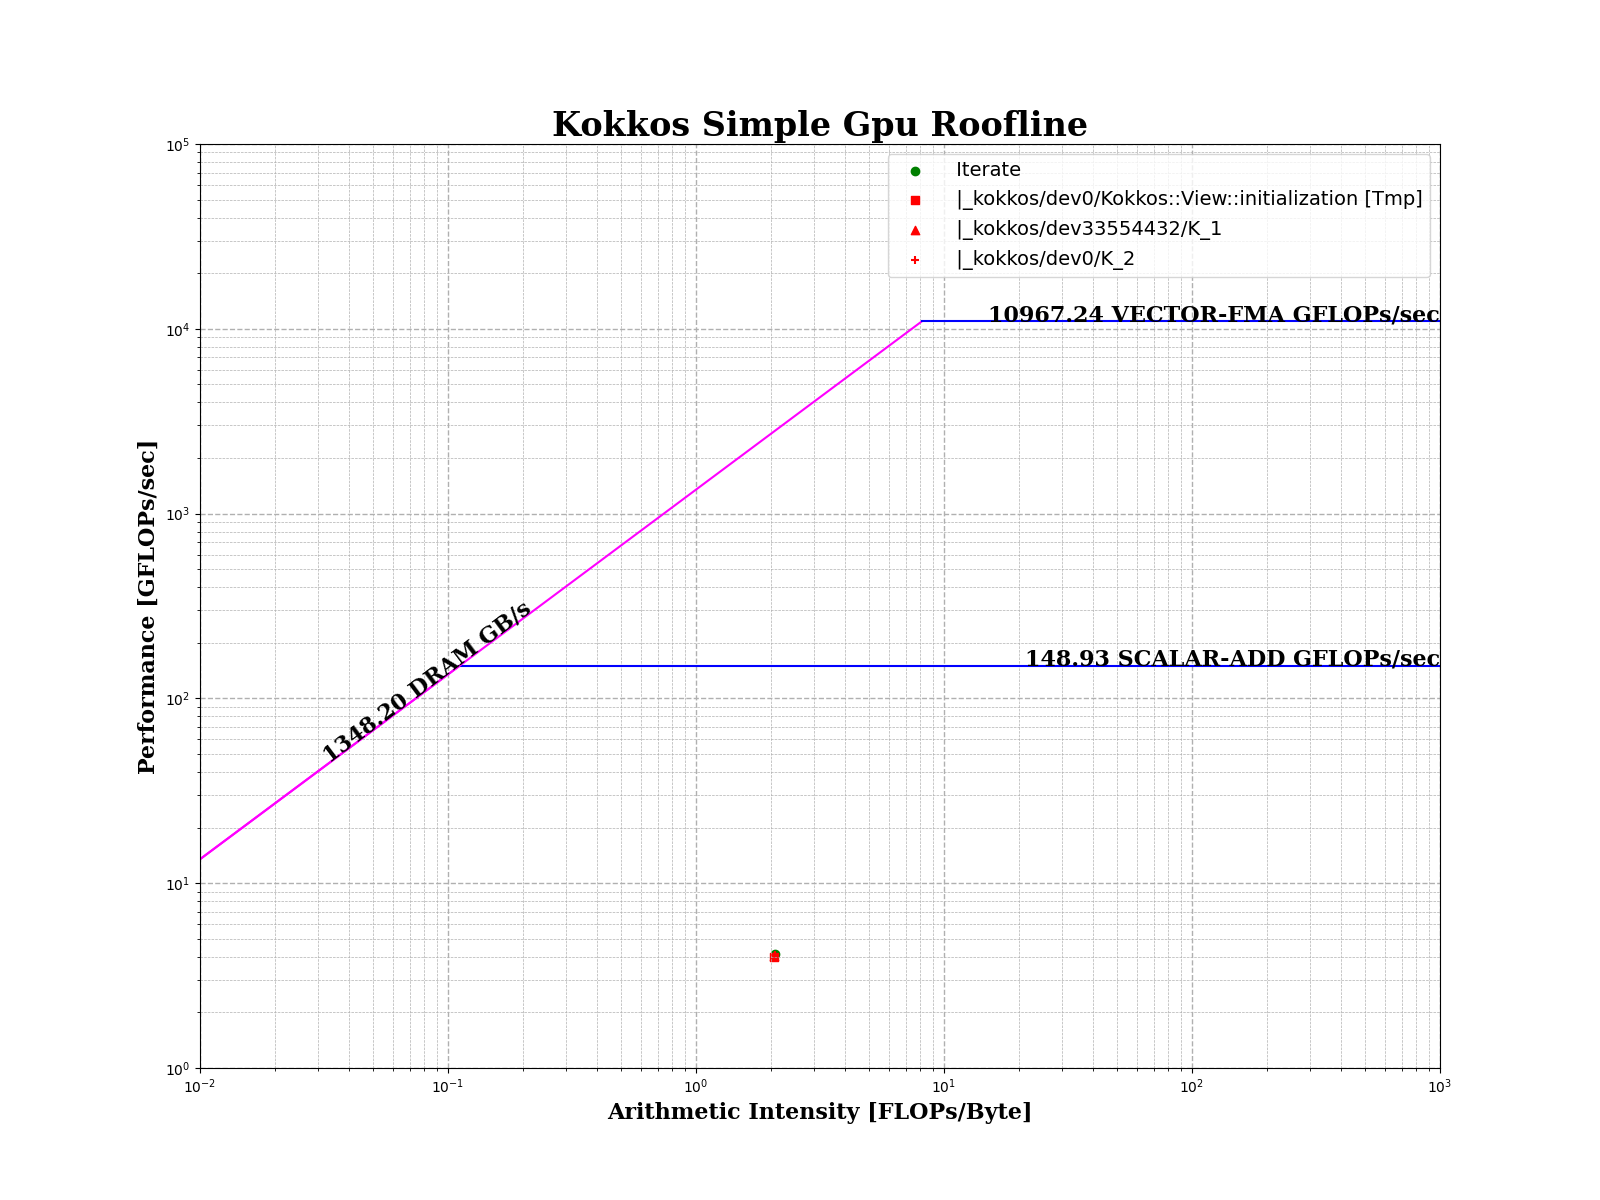
\includegraphics[width=\textwidth]{../figures/tools-simple-example-timemory.png}
\end{frame}

%==========================================================================

\begin{frame}[fragile]{Other}
  \begin{itemize}
    \item Caliper - Broad program analysis capabilities. UVM Profiling.
    \item HPCToolkit - Not a connector, but a sampling tool with great Kokkos support
  \end{itemize}

\end{frame}

%==========================================================================

\begin{frame}[fragile]{Connector Summary}
  \begin{itemize}
    \item Connectors inject Kokkos specific information into vendor and academic tools.
    \item Helps readability of profiles.
    \item Removes your need to put vendor specific instrumentation in your code.
    \item Growing list of tools support Kokkos natively.
  \end{itemize}
\end{frame}

